\documentclass{article}
\usepackage{iclr2024_conference,times}

\input{math_commands.tex}

\usepackage{hyperref}
\usepackage{url}
\usepackage{booktabs}
\usepackage{graphicx}
\usepackage{multirow}
\usepackage{amsmath,amssymb}
\usepackage{xcolor}
\usepackage{array}
\usepackage{enumitem}

\title{Denoising Autoencoders for Parkinson's Disease\\
Wrist IMU Signals: Architecture Comparison and Ablations}

\author{%
  Wanghley Soares Martins$^{1}$ \And Yibei Gou$^{1}$ \\
  $^{1}$Department of Electrical and Computer Engineering, Duke University \\
  \texttt{\{wanghley.martins,\;yibei.gou\}@duke.edu}
}

\newcommand{\fix}{\marginpar{FIX}}
\newcommand{\new}{\marginpar{NEW}}
\newcommand{\tremorMAE}{\text{TremorMAE}}

\iclrfinalcopy
\begin{document}

\maketitle

\begin{abstract}
We design, implement, and systematically compare five denoising autoencoder
architectures---FC, 1D-CNN, LSTM, UNet-1D, and patch-based Transformer---
applied to 6-channel wrist IMU recordings from the PADS Parkinson's Disease
Smartwatch Dataset \citep{varghese2023pads}.
Training uses a hybrid MSE\,+\,spectral-$L_1$ loss; evaluation uses MSE,
SNR improvement (SNRi), and a tremor-band power MAE (4--6\,Hz).
Five experiments cover architecture comparison, latent-dimension ablation,
noise-level robustness, noise-type cross-evaluation, and hyperparameter
search.
A clear divide governed by \emph{skip connections} emerges: UNet-1D and
Transformer both reach MSE\,$\approx 0.004$ and SNRi\,$\approx +5.4$\,dB,
while FC, CNN, and LSTM record negative SNRi ($-7$ to $-9$\,dB) and inflate
tremor-band distortion by 118--168$\times$.
\end{abstract}

% ════════════════════════════════════════════════════════════════════
\section{Introduction}
\label{sec:intro}

Parkinson's Disease (PD) resting tremor (4--6\,Hz) is a primary clinical
marker for diagnosis and therapy monitoring.
Consumer smartwatches record 6-axis wrist IMU data continuously, but the raw
signals are contaminated by motion artifacts, sensor dropout, ambient
vibrations, and electronic noise that can mask the tremor signature.
Classical spectral filters apply fixed operations that cannot adapt to
subject-specific, non-stationary corruption; learned denoising can in
principle adapt to the signal manifold.

We treat the problem as a \emph{reconstruction task}: given a noisily
corrupted window $\vx_{\text{noisy}} \in \mathbb{R}^{6\times1024}$,
recover the clean signal $\vx$.
The models are trained \emph{self-supervisedly}---clean signals from the PADS
dataset are used as ground truth and corrupted on-the-fly during training,
so no paired noisy recordings are needed.

Our contributions are: (i) a complete end-to-end pipeline for multi-channel
wrist IMU denoising on PADS \footnote{Codebase: \url{https://github.com/Wanghley/parkinsons-imu-denoising}}; (ii) a domain-specific TremorMAE metric that
measures distortion in the clinically critical band; (iii) a systematic
five-experiment comparison identifying skip connections as the key architectural
requirement.

% ════════════════════════════════════════════════════════════════════
\section{Dataset and Preprocessing}
\label{sec:data}

\textbf{PADS dataset.}
The PADS Parkinson's Disease Smartwatch Dataset \citep{varghese2023pads}
contains recordings from 355 subjects (276 PD patients, 79 healthy controls)
wearing bilateral Apple Watch Series~4 devices at 100\,Hz.
Each subject performed 11 structured motor tasks
(relaxed rest, outstretched hold, finger-to-nose, drinking, etc.);
each task yields a 1024-sample (10.24\,s) window stored as a CSV with columns
\texttt{Accel\_{X,Y,Z}}, \texttt{Gyro\_{X,Y,Z}}.

\textbf{Preprocessing.}
(1)~The first 50 samples are discarded (haptic notification artifact).
(2)~Windows of $L=1024$ are extracted with 87.5\% overlap during training and
non-overlapping during evaluation.
(3)~Per-channel z-score normalisation is computed on the training split only
and applied identically to all splits (no data leakage).

\textbf{Subject-level split.}
Subjects are shuffled (seed 42) and split 80/10/10 by identity, preventing
patient-level memorisation:
$\approx$197 training / $\approx$25 validation / $\approx$25 test subjects,
yielding $\approx$10\,300 / 520 / 520 windows respectively.

% ════════════════════════════════════════════════════════════════════
\section{Noise Models}
\label{sec:noise}

All corruptions are applied on-the-fly to $(B,6,1024)$ tensors.
\textbf{Gaussian} ($\sigma=0.1$): additive white noise,
$\vx_\text{noisy}=\vx+\boldsymbol{\varepsilon}$,
$\boldsymbol{\varepsilon}\!\sim\!\mathcal{N}(0,\sigma^2\mathbf{I})$.
\textbf{Masking} ($p=0.1$, $L_\text{mask}=20$): contiguous 200\,ms dropout
segments applied identically across all 6 channels (physical contact loss).
\textbf{Impulse} ($p=0.05$, $A=3.0$): random large-amplitude spikes.
\textbf{Sinusoidal} ($f=5$\,Hz, $A=0.3$): periodic tone directly overlapping
the tremor band.

% ════════════════════════════════════════════════════════════════════
\section{Model Architectures}
\label{sec:models}

All five learned architectures share the encoder-decoder paradigm with a
$d_z$-dimensional bottleneck (default $d_z=64$), input/output shape
$(B,6,1024)$, and the same training procedure.
A non-parametric wavelet baseline is included for reference.

\textbf{FC autoencoder.}
The full $6\!\times\!1024=6144$-element window is flattened and encoded via
$6144\!\to\!256\!\to\!128\!\to\! d_z$ (ReLU, Dropout 0.2); decoding mirrors
in reverse.
No temporal structure is assumed.
\textbf{3.23M params.}

\textbf{1D-CNN autoencoder.}
Four strided Conv1d encoder stages (kernel 3, stride 2, padding 1; channels
$6\!\to\!32\!\to\!64\!\to\!128\!\to\!256$; ReLU, Dropout 0.1) halve the
temporal resolution at each stage; ConvTranspose1d mirrors in the decoder.
A linear layer projects the final $(256,64)$ feature map to $d_z$.
\textbf{2.42M params.}

\textbf{LSTM autoencoder.}
Input is transposed to $(B,L,C)$.
Encoder: 2-layer bidirectional LSTM (hidden 128); the \emph{terminal}
forward and backward hidden states are concatenated ($(B,256)$) and linearly
projected to $d_z$---avoiding the vanishing-gradient failure of mean pooling
over 1024 steps.
Decoder: $d_z$ initialises a 2-layer unidirectional LSTM (hidden 128) fed
zero inputs; a linear head maps hidden states to 6 output channels.
\textbf{787K params.}

\textbf{UNet-1D autoencoder.}
A CNN encoder-decoder augmented with \emph{skip connections} that concatenate
encoder feature maps directly into the matching decoder stage at four spatial
scales.
The decoder receives both the bottleneck latent and full-resolution local
features, reducing denoising to a residual problem at each scale
\citep{ronneberger2015unet,he2016deep}.
\textbf{2.46M params.}

\textbf{Patch Transformer autoencoder.}
The signal is divided into $N_P=128$ non-overlapping 8-sample patches; each
patch ($\in\mathbb{R}^{48}$) is linearly projected to $d_\text{model}=128$.
Two Pre-LayerNorm Transformer encoder layers \citep{vaswani2017attention}
($n_\text{heads}=4$, $d_\text{ff}=256$, dropout 0.1) process the token
sequence; mean pooling and a linear layer give $d_z$.
The decoder tiles $d_z$ back to 128 tokens, adds positional embeddings, and
refines with two further encoder layers before projecting each token to a
8-sample patch.
Critically, the full encoder token sequence is \emph{added} to the decoder
input (patch-level skip bypass), giving the Transformer access to per-patch
detail without routing it through the bottleneck.
\textbf{575K params.}

\textbf{Wavelet baseline (db8, level 4).}
Donoho--Johnstone soft-thresholding \citep{donoho1995wavelet}: MAD-based
universal threshold applied to DWT detail subbands per channel; no training.
\textbf{0 params.}

% ════════════════════════════════════════════════════════════════════
\section{Training Procedure and Metrics}
\label{sec:training}

\textbf{Hybrid loss.}
\begin{equation}
  \mathcal{L}(\vtheta)
  = \|\hat{\vx}-\vx\|_2^2
  + \alpha\,\bigl\||\mathcal{F}(\hat{\vx})|-|\mathcal{F}(\vx)|\bigr\|_1,
  \quad \alpha=0.1.
  \label{eq:loss}
\end{equation}
The spectral $L_1$ term penalises power-spectrum deviations, explicitly
preserving tremor-band content that MSE alone can over-smooth.

\textbf{Optimisation.}
Adam \citep{kingma2015adam} with weight decay $10^{-5}$; gradient clipping
(max $L_2$ norm 1.0); \texttt{ReduceLROnPlateau} (factor 0.5, patience 10,
monitored on validation hybrid loss); batch 128; AMP (FP16) on CUDA.
Best checkpoint by validation loss is retained.

\textbf{Metrics.}
MSE (mean squared error); SNRi\,=\,SNR$_\text{out}$\,$-$\,SNR$_\text{in}$
(positive $=$ model improves over noisy input);
\emph{TremorMAE}\,=\,mean absolute error of the 4--6\,Hz band power
$P_{4\text{-}6}(\vx)=\sum_{f\in[4,6]\text{Hz}}|\mathcal{F}(\vx)[f]|^2$.
A model with low MSE but high TremorMAE is clinically harmful.

% ════════════════════════════════════════════════════════════════════
\section{Experiments and Results}
\label{sec:experiments}

% ────────────────────────────────────────────
\subsection{Experiment 1: Hyperparameter Search}
\label{sec:exp-hyperparam}

\textbf{Setup.} Grid search over
lr\,$\in\{10^{-4},5\!\times\!10^{-4},10^{-3}\}$ and
batch\,$\in\{32,64,128\}$ using CNN, 20 epochs, Gaussian noise.

\begin{table}[h]
\caption{Best validation hybrid loss (CNN, 20 epochs). Best cell \textbf{bold}.}
\label{tab:hyperparam}
\vspace{-4pt}
\begin{center}
\small
\begin{tabular}{lccc}
\toprule
\textbf{LR} & \textbf{Batch 32} & \textbf{Batch 64} & \textbf{Batch 128} \\
\midrule
$1\times10^{-4}$ & 2.049 & 2.048 & 2.079 \\
$5\times10^{-4}$ & \textbf{1.657} & 1.824 & 1.844 \\
$1\times10^{-3}$ & 1.702 & 1.789 & 1.778 \\
\bottomrule
\end{tabular}
\end{center}
\vspace{-6pt}
\end{table}

\begin{figure}[h]
\begin{center}
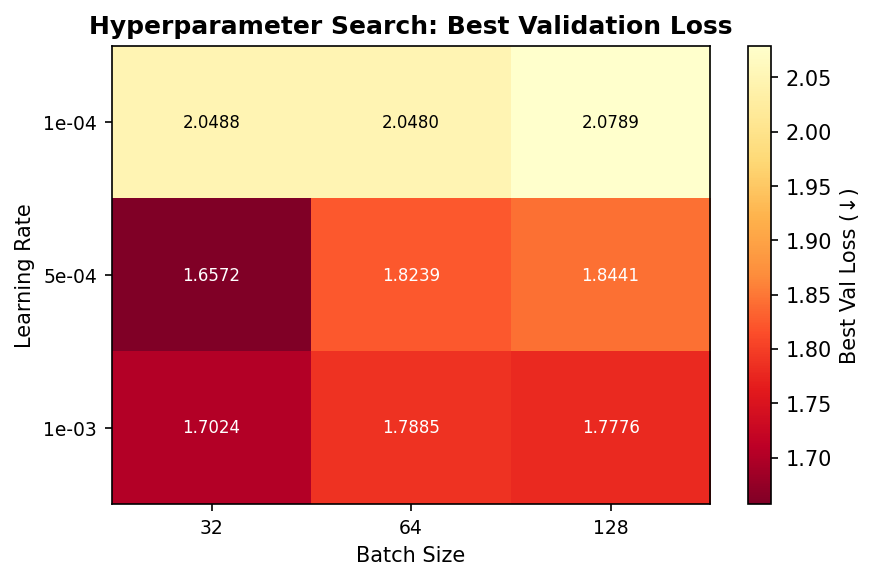
\includegraphics[width=0.82\linewidth]{assets/hyperparam_search.png}
\end{center}
\vspace{-6pt}
\caption{Hyperparam grid (CNN, 20 ep). Darker\,=\,lower loss. Optimal: lr\,$=5\!\times\!10^{-4}$, batch 32.}
\label{fig:hyperparam}
\vspace{-4pt}
\end{figure}

The optimal cell (lr\,$=5\!\times\!10^{-4}$, batch 32, loss 1.657) shows that
learning rate dominates over batch size: the $10^{-4}$ row converges too
slowly; $5\!\times\!10^{-4}$ and $10^{-3}$ behave similarly.
Main experiments use lr\,$=10^{-3}$ with \texttt{ReduceLROnPlateau}, which
adaptively anneals into the identified optimal range.

% ────────────────────────────────────────────
\subsection{Experiment 2: Architecture Comparison}
\label{sec:exp-arch}

\textbf{Setup.}
All six models evaluated on Gaussian noise ($\sigma=0.1$), held-out test split
(35 subjects, 979 windows).
Learned models: 100 epochs, lr\,$=10^{-3}$, batch 128.
Wavelet: applied directly.
SNR$_\text{in}\approx9.41$\,dB for all models.

\begin{table}[h]
\caption{Architecture comparison ($\sigma=0.1$, 100 epochs).
TremorMAE$_\text{in}$\,=\,noisy-signal baseline.
\textbf{Bold}: best learnable model. $\dagger$\,non-trainable.}
\label{tab:arch-results}
\vspace{-4pt}
\begin{center}
\small
\begin{tabular}{lcccc}
\toprule
\textbf{Model} & \textbf{MSE$\downarrow$} & \textbf{SNRi$\uparrow$} &
  \multicolumn{2}{c}{\textbf{TremorMAE (Hz$^2$)}} \\
\cmidrule(lr){4-5}
& & & In & Out$\downarrow$ \\
\midrule
FC          & 1.509 & $-8.96$ & 0.54 & \phantom{0}87.46 \\
CNN         & 0.831 & $-7.23$ & 0.54 & \phantom{0}63.85 \\
LSTM        & 1.542 & $-8.89$ & 0.53 & \phantom{0}90.02 \\
UNet-1D     & \textbf{0.004} & $+$\textbf{5.34} & 0.55 & \phantom{00}\textbf{0.68} \\
Transformer & \textbf{0.004} & $+$\textbf{5.46} & 0.55 & \phantom{00}\textbf{0.64} \\
\midrule
Wavelet$^\dagger$ & 0.031 & $+0.53$ & 0.55 & \phantom{0}17.69 \\
\bottomrule
\end{tabular}
\end{center}
\vspace{-6pt}
\end{table}

\textbf{Analysis.}
Table~\ref{tab:arch-results} reveals a binary split.
UNet-1D and Transformer both reach MSE\,$\approx 0.004$ and positive SNRi
($+5.34$ and $+5.46$\,dB), a $\mathbf{200\times}$ MSE advantage over the
bottleneck-only group (MSE 0.831--1.542, SNRi $-7$ to $-9$\,dB).
Clinically, FC/CNN/LSTM inflate TremorMAE by \textbf{118--168$\times$}
(0.54\,$\to$\,64--90\,Hz$^2$), making downstream tremor assessment unreliable.
UNet/Transformer keep TremorMAE below 0.68\,Hz$^2$.
The Wavelet baseline sits between groups: SNRi\,$+0.53$\,dB is positive but
modest; TremorMAE\,17.69\,Hz$^2$ is 26$\times$ worse than Transformer because
the MAD threshold does not specifically target the 4--6\,Hz DWT scale.

\textbf{Why the divide?}
UNet-1D concatenates encoder feature maps at 4 spatial scales directly into
the decoder---the decoder needs only to learn the residual noise, not
reconstruct the signal from scratch.
The Transformer adds the full 128-token encoder patch sequence to its decoder
input (patch-level skip), providing per-patch bypass of the 64-dim bottleneck.
FC, CNN, and LSTM route all 6144 inputs through 64 numbers; the resulting
information loss exceeds the noise power, giving negative SNRi.

\begin{figure}[h]
\begin{center}
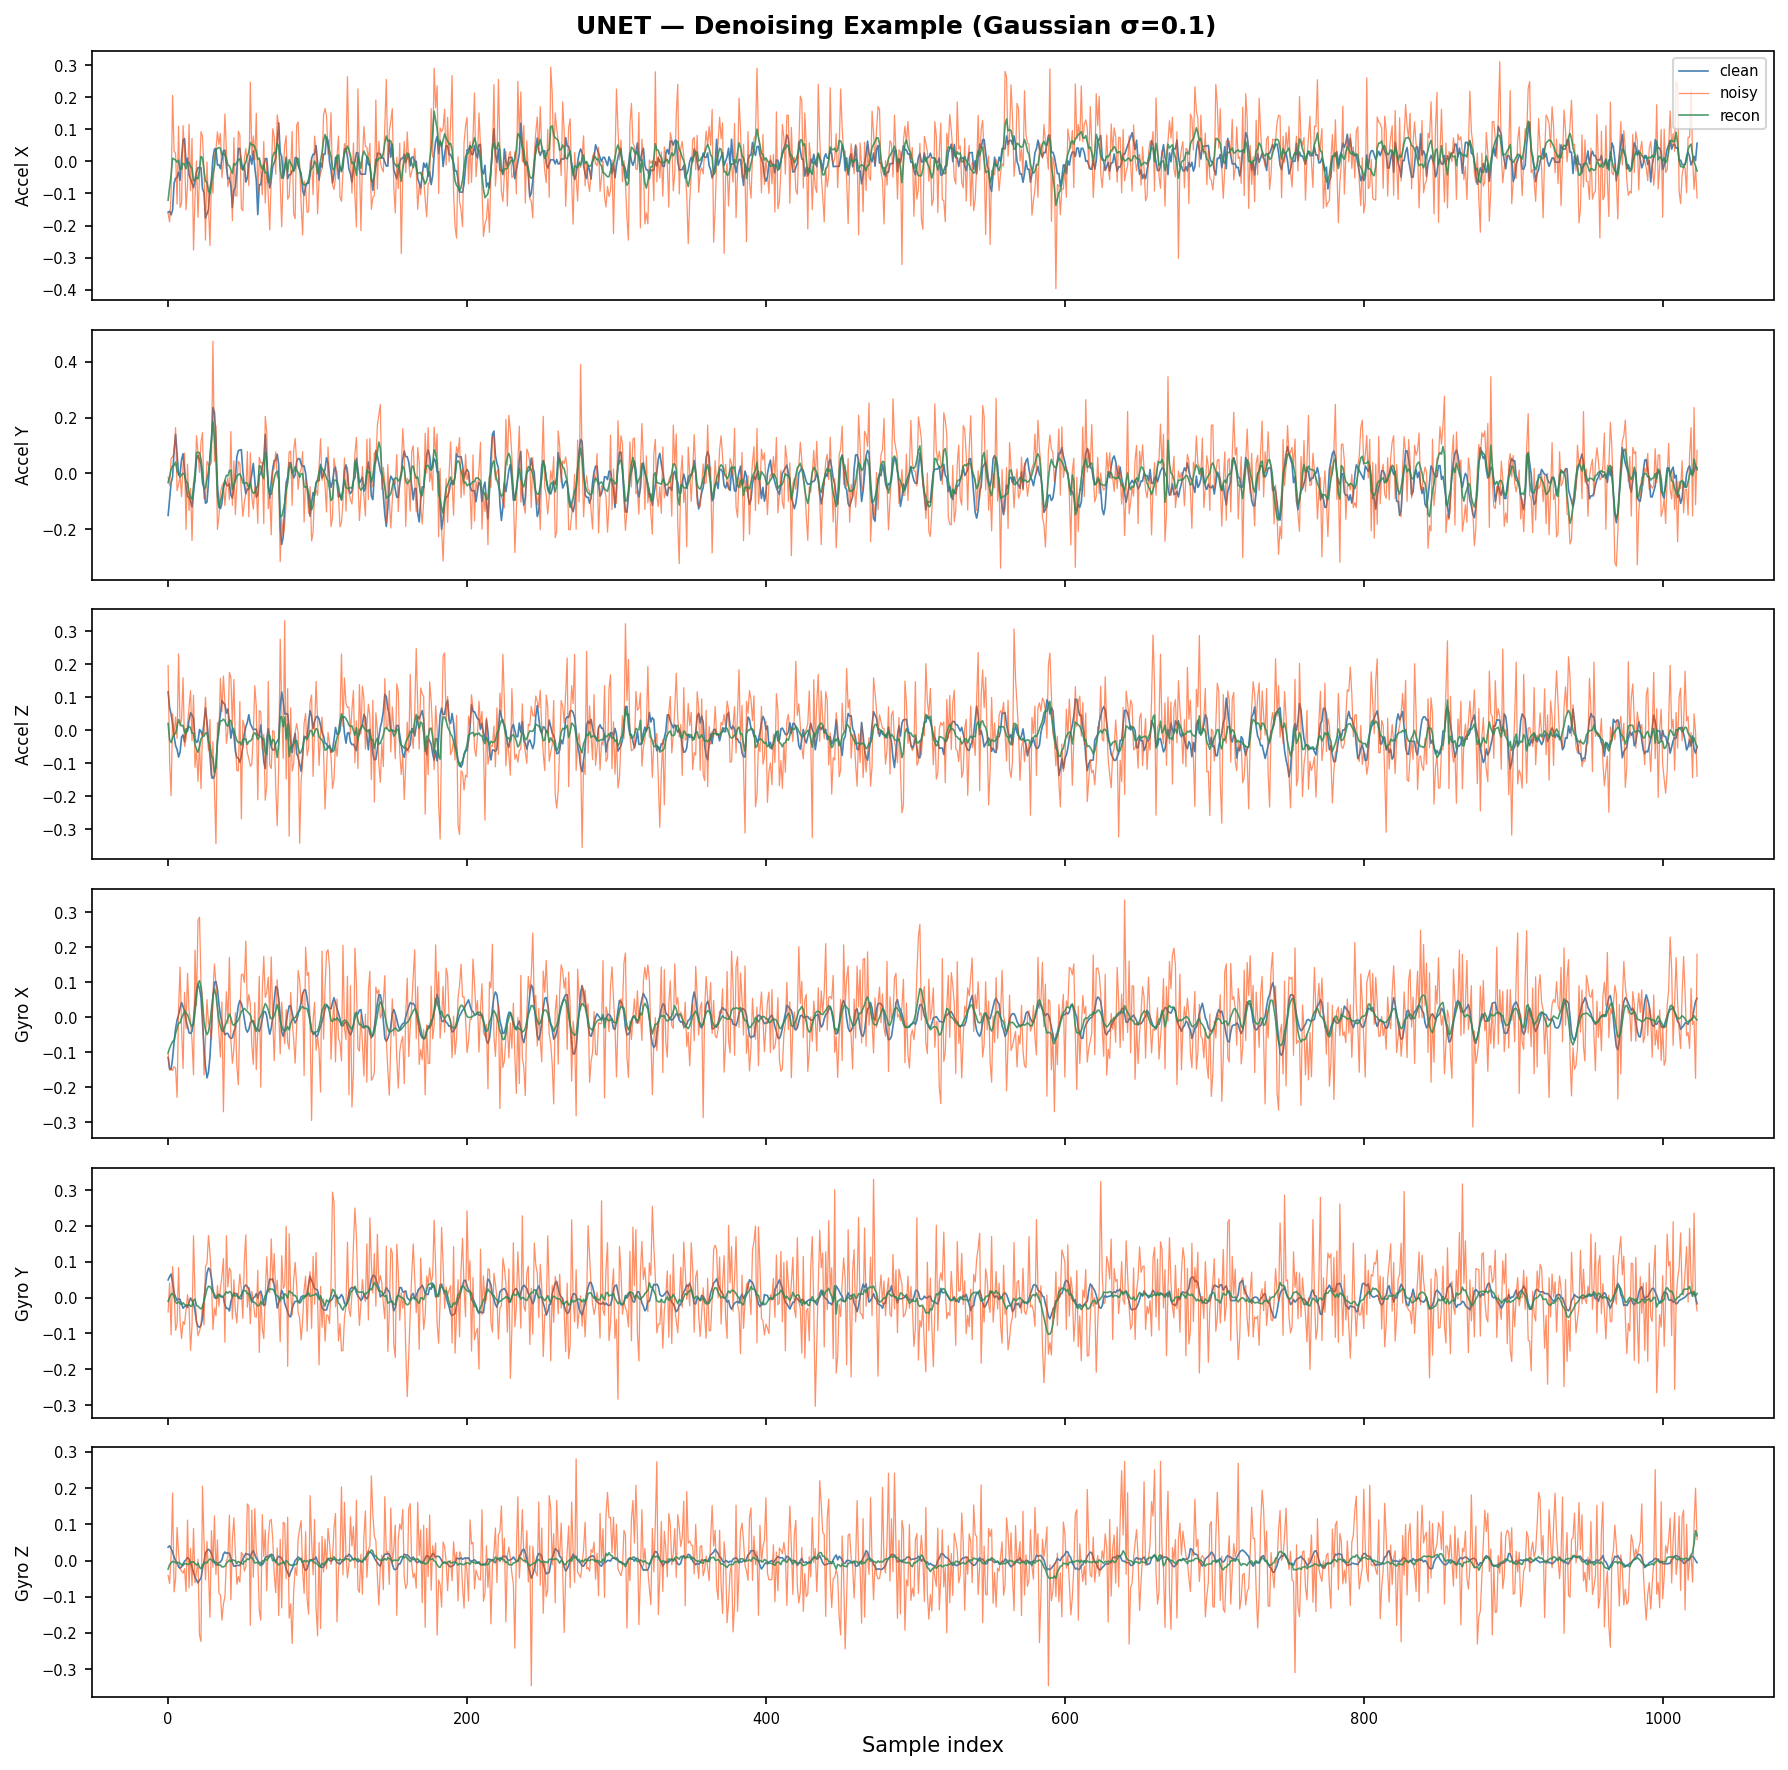
\includegraphics[width=0.49\linewidth]{assets/unet_reconstruction.png}
\hfill
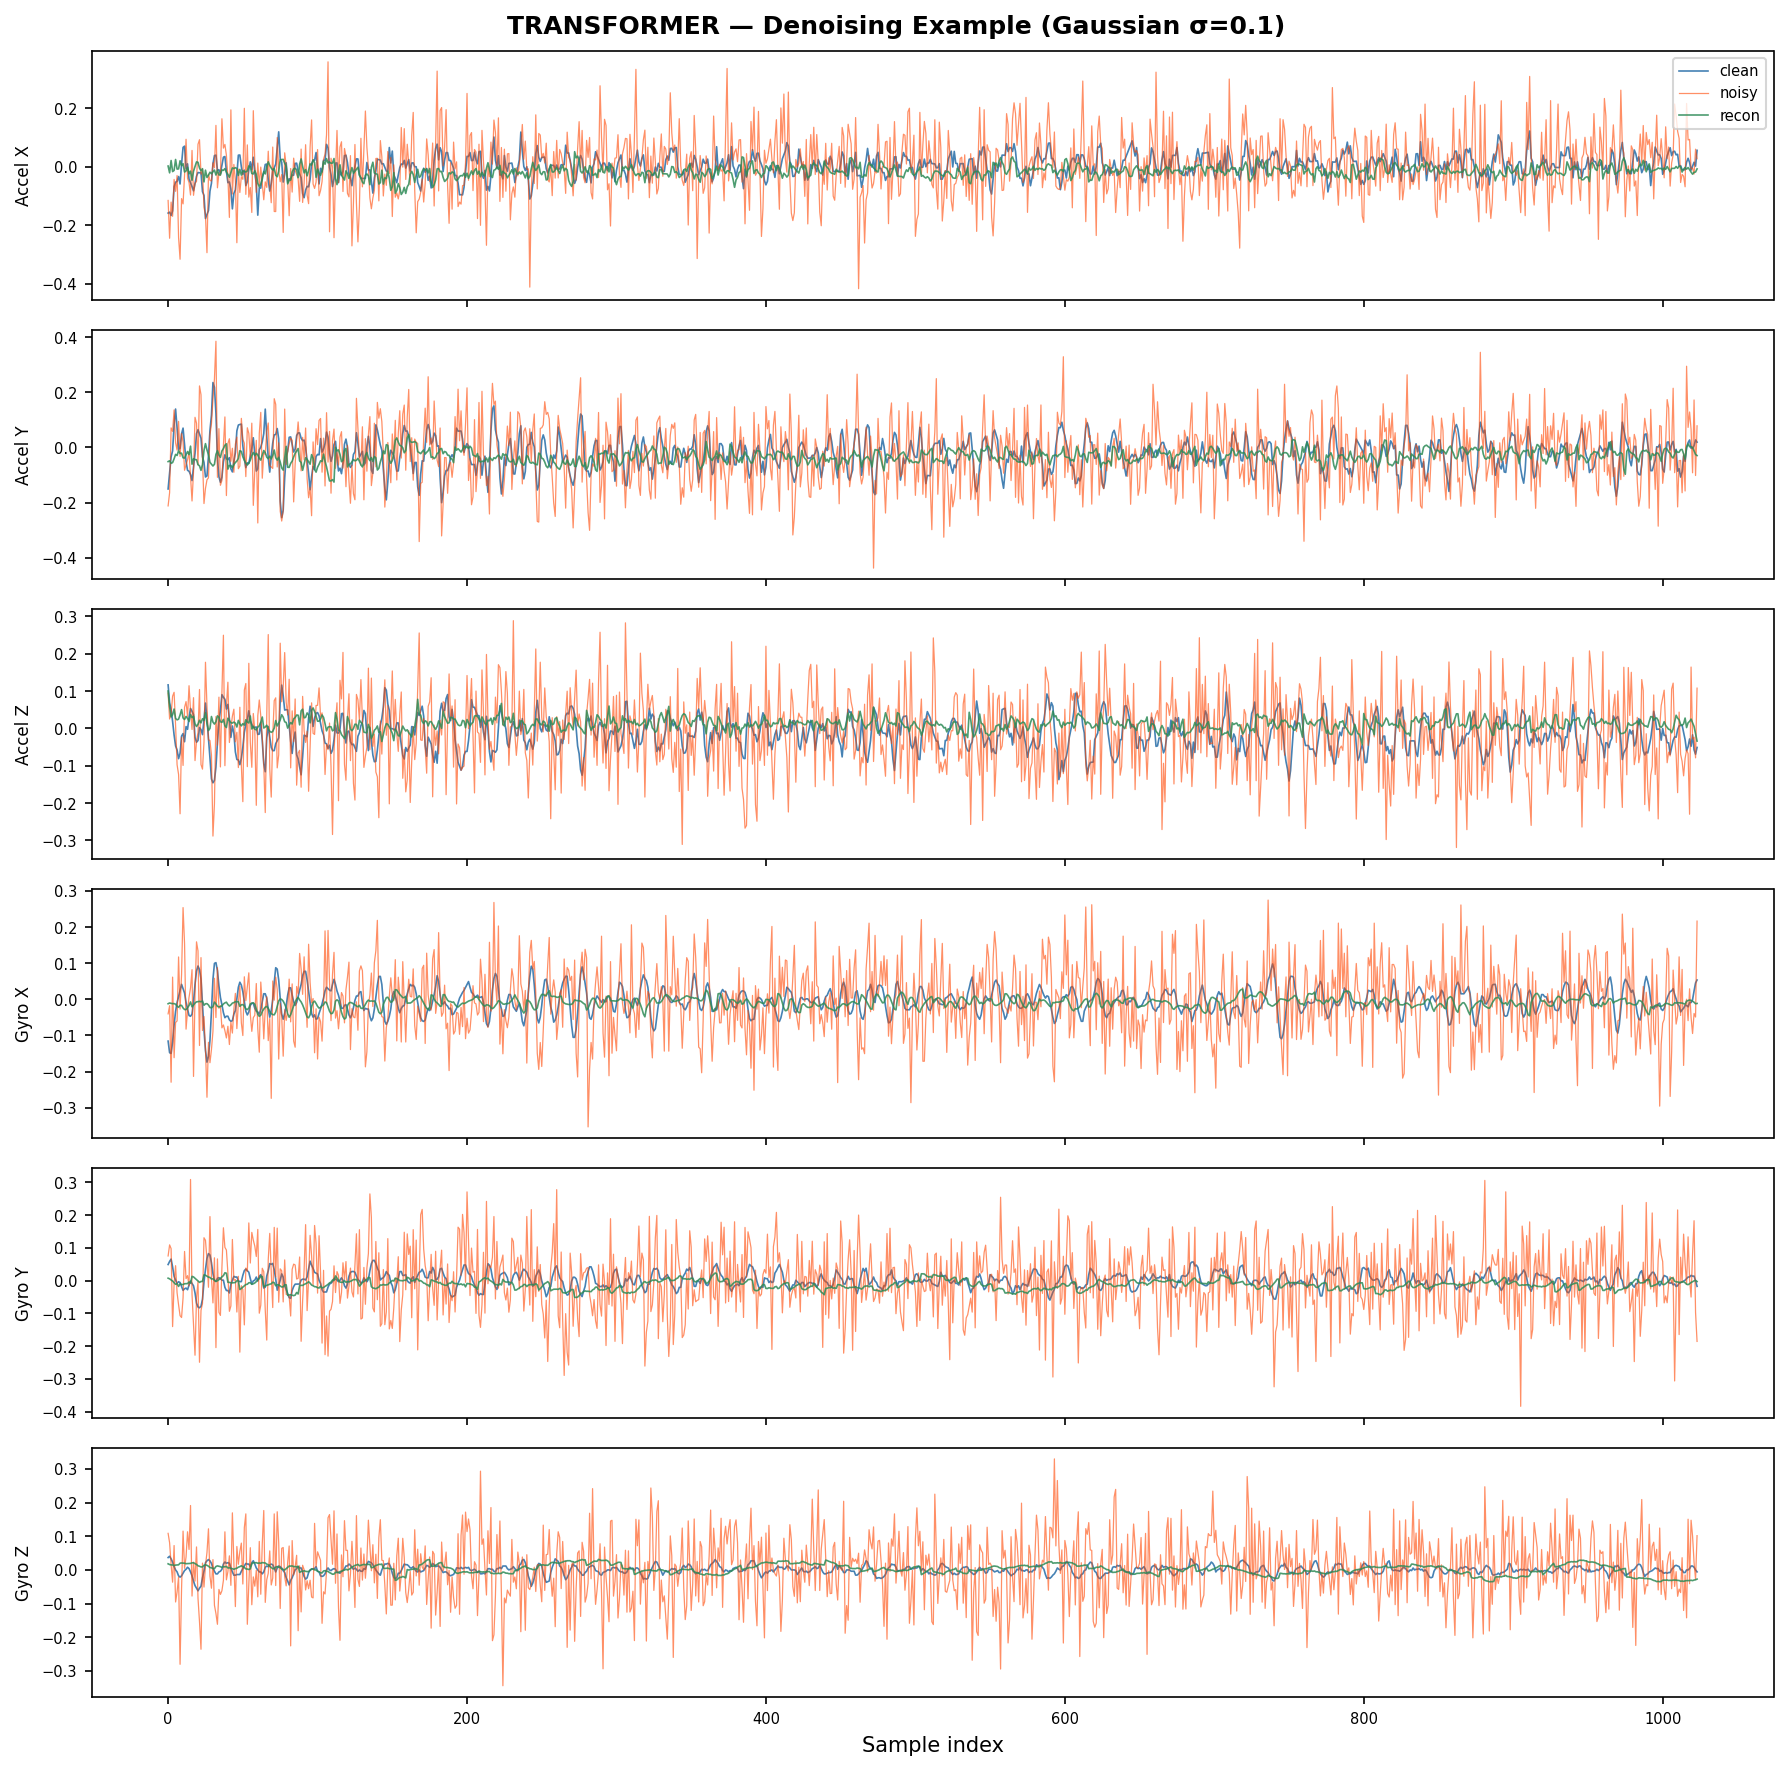
\includegraphics[width=0.49\linewidth]{assets/transformer_reconstruction.png}
\end{center}
\vspace{-4pt}
\caption{Reconstructions (6-ch, 1024 samples, $\sigma=0.1$).
\textbf{Left}: UNet-1D. \textbf{Right}: Transformer.
Blue = clean, red = noisy, green = reconstruction.
Both track the clean signal faithfully across all 6 channels.}
\label{fig:recon-good}
\vspace{-4pt}
\end{figure}

\begin{figure}[h]
\begin{center}
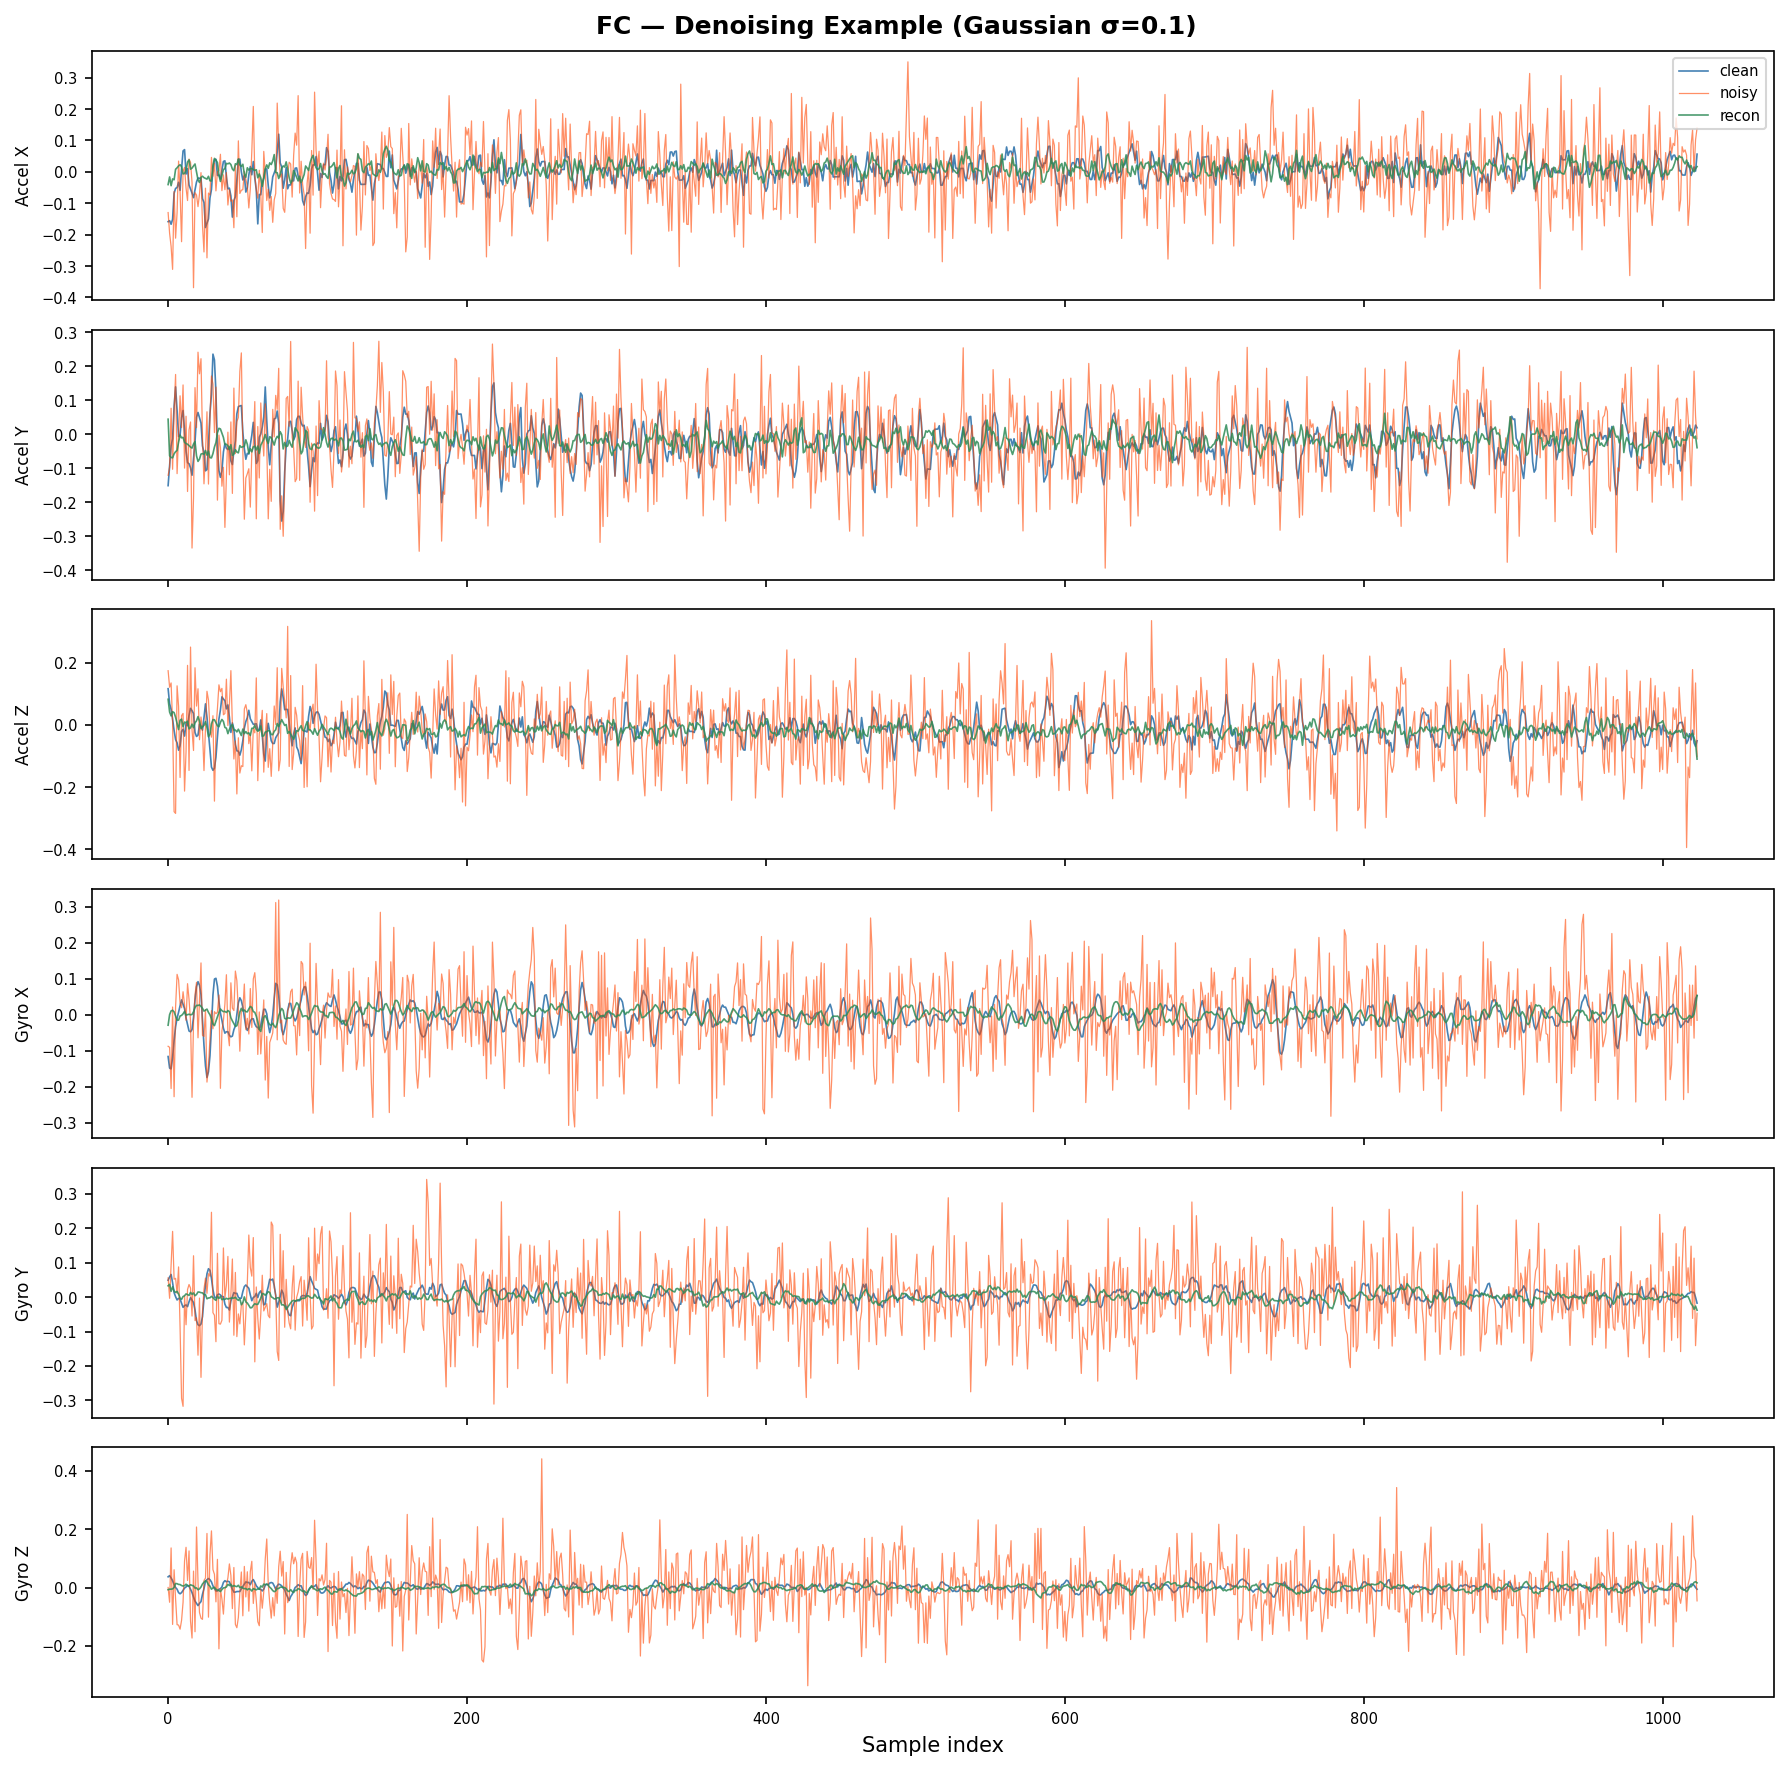
\includegraphics[width=0.49\linewidth]{assets/fc_reconstruction.png}
\hfill
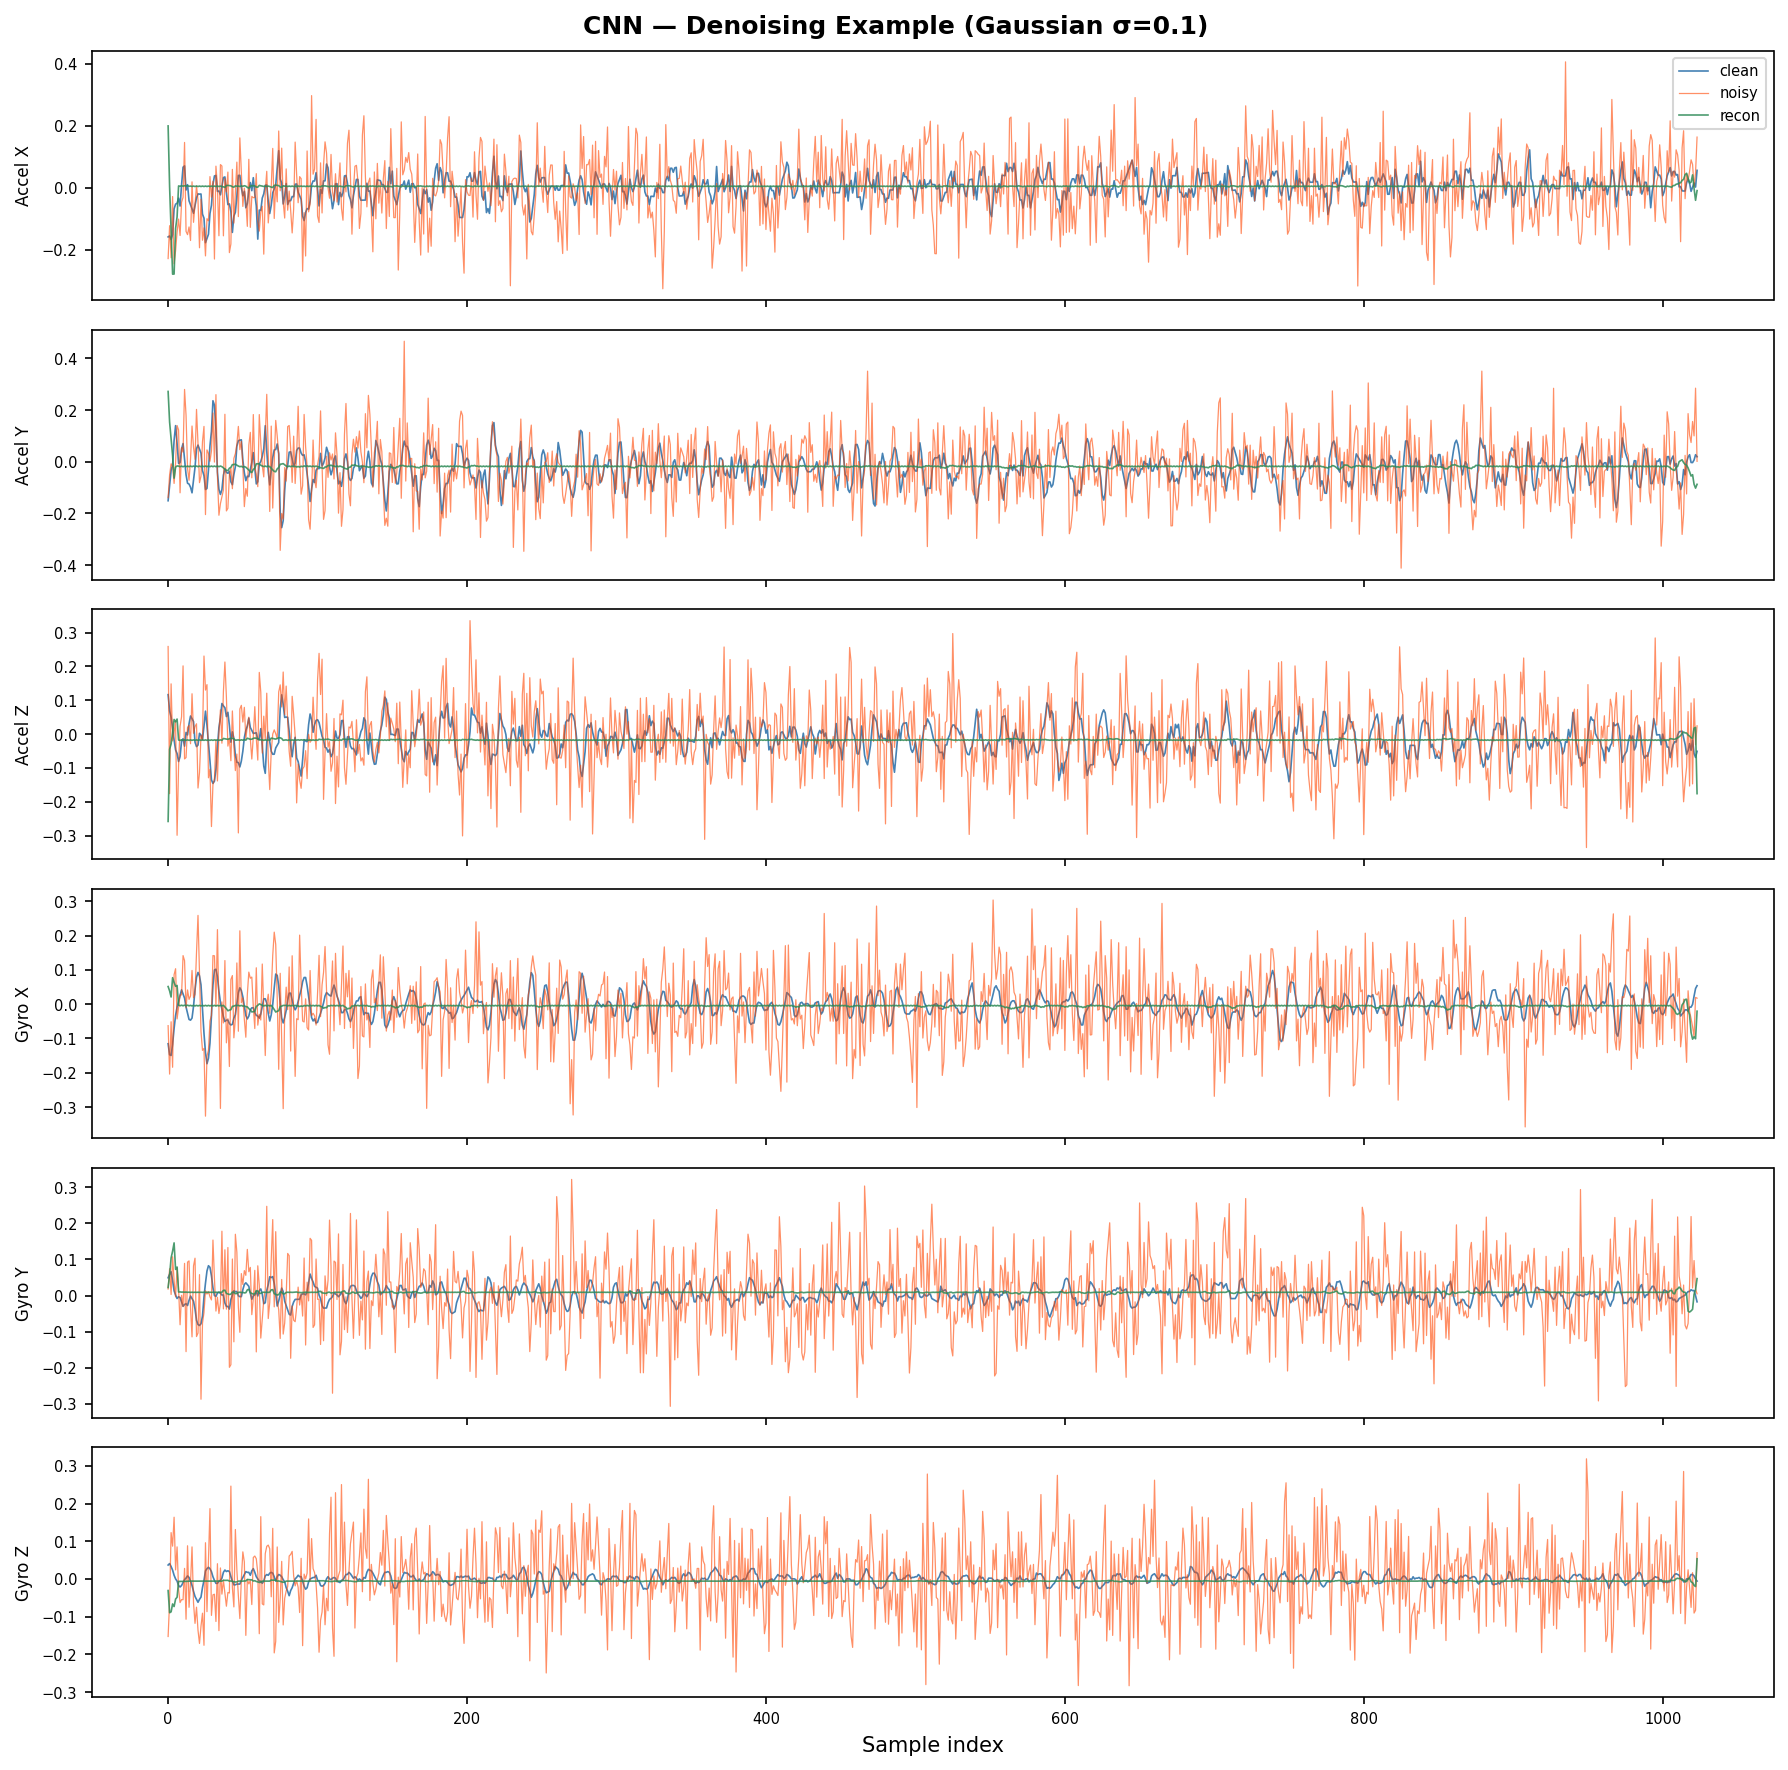
\includegraphics[width=0.49\linewidth]{assets/cnn_reconstruction.png}
\end{center}
\vspace{-4pt}
\caption{Bottleneck-only models: \textbf{Left} FC (TremorMAE 87\,Hz$^2$);
\textbf{Right} CNN (TremorMAE 64\,Hz$^2$). Both erase fine oscillation detail.}
\label{fig:recon-bad}
\vspace{-4pt}
\end{figure}

% ────────────────────────────────────────────
\subsection{Experiment 3: Latent Dimension Sweep}
\label{sec:exp-latent}

\textbf{Setup.} All six architectures evaluated at
$d_z \in \{8,16,32,64,128,256\}$, 50 epochs each, Gaussian noise, all other
hyperparameters fixed.

\begin{table}[h]
\caption{MSE vs.\ latent dimension (50 epochs). Wavelet is constant (no $d_z$).}
\label{tab:latent}
\vspace{-4pt}
\begin{center}
\small
\begin{tabular}{lcccccc}
\toprule
\textbf{Model} & $d_z{=}8$ & 16 & 32 & 64 & 128 & 256 \\
\midrule
FC      & 1.752 & 1.627 & 1.586 & 1.579 & 1.583 & 1.556 \\
CNN     & 1.418 & 1.240 & 1.042 & 0.884 & 0.826 & 0.839 \\
LSTM    & 1.895 & 1.766 & 1.808 & 1.821 & 1.780 & 1.828 \\
UNet-1D & 0.0050 & 0.0051 & 0.0057 & 0.0051 & 0.0050 & 0.0051 \\
Transf. & 0.0044 & 0.0043 & 0.0043 & 0.0043 & 0.0043 & 0.0043 \\
Wavelet & \multicolumn{6}{c}{0.031 (constant)} \\
\bottomrule
\end{tabular}
\end{center}
\vspace{-6pt}
\end{table}

\begin{figure}[h]
\begin{center}
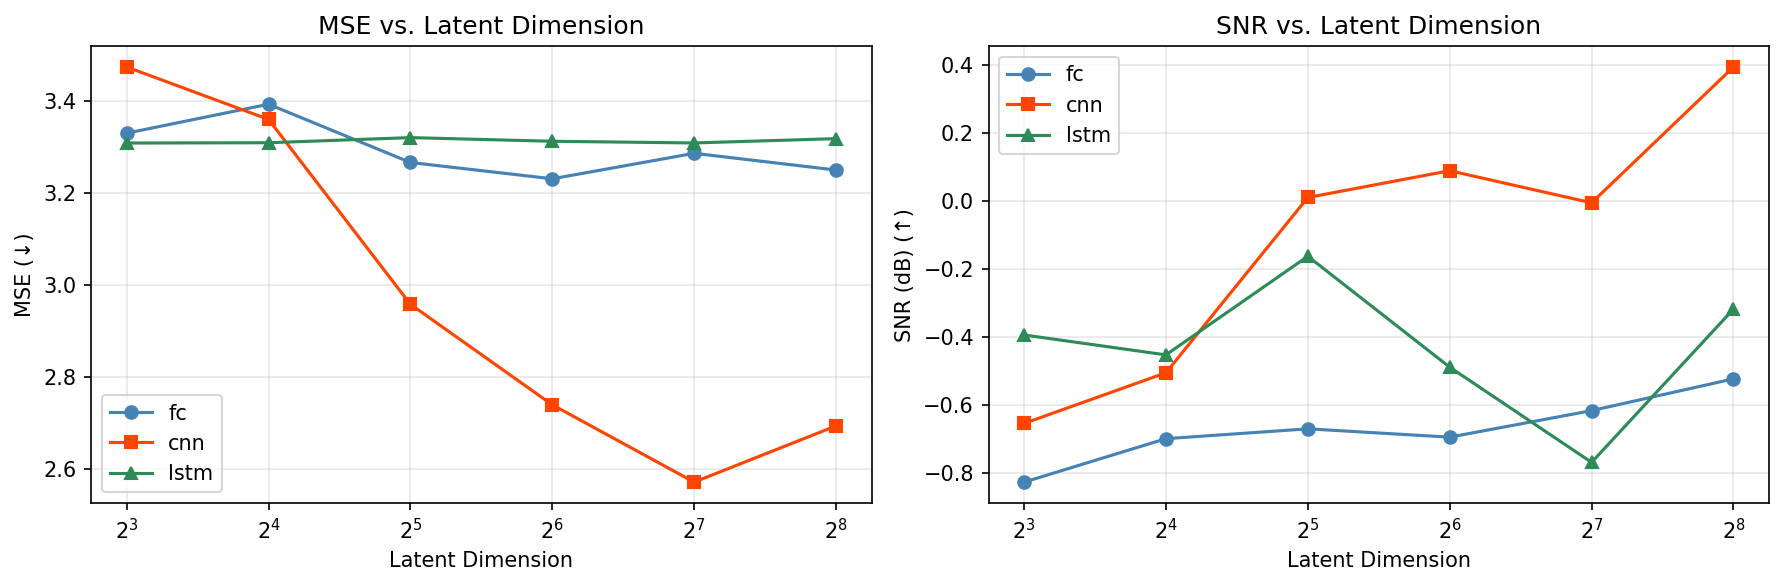
\includegraphics[width=0.9\linewidth]{assets/latent_dim_sweep.png}
\end{center}
\vspace{-6pt}
\caption{SNR$_\text{out}$ (dB) vs.\ $d_z$ for all architectures (50 epochs).
UNet/Transformer are flat near 14\,dB; CNN improves monotonically;
FC and LSTM are flat at low performance.}
\label{fig:latent}
\vspace{-4pt}
\end{figure}

\textbf{Analysis.}
Three distinct behaviours emerge.
\emph{Skip-connection models are bottleneck-invariant.}
UNet-1D MSE varies by $<$15\% across the full 32$\times$ $d_z$ range;
Transformer by $<$3\%.
Their bypass paths carry per-patch or per-scale detail regardless of $d_z$.
\emph{CNN is bottleneck-limited.}
MSE drops monotonically from 1.418 at $d_z=8$ to 0.826 at $d_z=128$ (42\%
improvement), confirming the encoder learns useful representations that
wider bottlenecks can preserve.
Skip connections would remove this dependency entirely.
\emph{FC and LSTM are not bottleneck-limited.}
Both are nearly flat across all $d_z$; their poor performance stems from
the absence of useful inductive bias (FC) and the difficulty of compressing
1024 recurrent steps into a vector (LSTM), not from a capacity bottleneck.

% ────────────────────────────────────────────
\subsection{Experiment 4: Noise Robustness}
\label{sec:exp-noise}

\textbf{Setup.}
All architectures trained at $\sigma_\text{train}=0.1$ (100 epochs),
evaluated at $\sigma_\text{test} \in \{0.05,\,0.10,\,0.20,\,0.40\}$.

\begin{table}[h]
\caption{SNRi (dB) across test noise levels (trained at $\sigma{=}0.1$).
\textbf{Bold}: positive (model improves over noisy input).}
\label{tab:noise-robust}
\vspace{-4pt}
\begin{center}
\small
\begin{tabular}{lcccc}
\toprule
\textbf{Model} & $\sigma{=}0.05$ & $\sigma{=}0.10$ & $\sigma{=}0.20$ & $\sigma{=}0.40$ \\
\midrule
FC      & $-14.96$ & $-8.95$ & $-2.93$ & $+$\textbf{3.09} \\
CNN     & $-13.42$ & $-7.26$ & $-1.28$ & $+$\textbf{4.42} \\
LSTM    & $-15.15$ & $-9.13$ & $-3.10$ & $+$\textbf{2.93} \\
UNet-1D & $+$\textbf{2.06} & $+$\textbf{5.52} & $+$\textbf{4.91} & $+$\textbf{3.06} \\
Transf. & $+$\textbf{1.23} & $+$\textbf{5.50} & $+$\textbf{4.39} & $+$\textbf{3.02} \\
Wavelet & $-3.04$ & $+$\textbf{0.52} & $+$\textbf{3.57} & $+$\textbf{6.14} \\
\bottomrule
\end{tabular}
\end{center}
\vspace{-6pt}
\end{table}

\begin{figure}[h]
\begin{center}
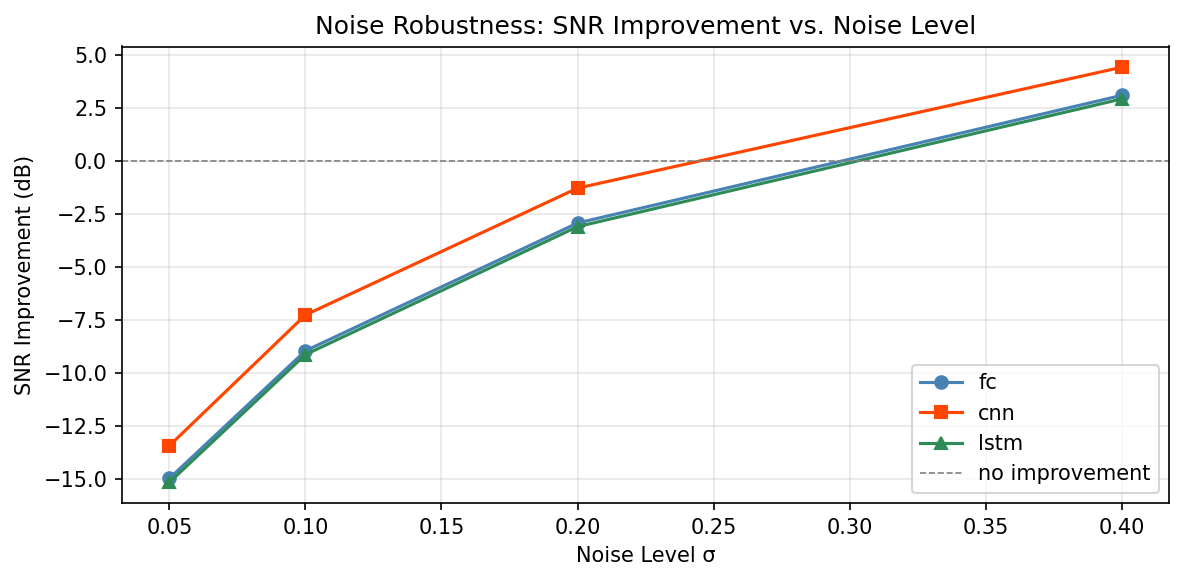
\includegraphics[width=0.88\linewidth]{assets/noise_robustness.png}
\end{center}
\vspace{-6pt}
\caption{SNRi vs.\ test $\sigma$ (all models trained at $\sigma=0.1$).
Dashed line: SNRi\,=\,0. Only UNet-1D and Transformer maintain positive
SNRi across the full range; FC/CNN/LSTM cross zero only at $\sigma=0.4$.}
\label{fig:noise-robust}
\vspace{-4pt}
\end{figure}

\textbf{Analysis.}
UNet-1D and Transformer are the only models with positive SNRi at every
tested $\sigma$, including the challenging low-noise regime
($\sigma=0.05$: $+2.06$ and $+1.23$\,dB).
Both peak near the training level ($\sigma=0.10$, $\approx+5.5$\,dB) and
degrade gracefully, consistent with a matched-filter interpretation.
FC, CNN, and LSTM cross positive SNRi only at $\sigma=0.40$, which exceeds
typical real-world wrist IMU artifact severity ($\sigma<0.2$).
The Wavelet baseline improves monotonically with $\sigma$
($-3.04\to+6.14$\,dB), eventually surpassing all bottleneck-only learned
models; its MAD threshold scales with noise level, giving natural
scale-adaptive behaviour.

% ────────────────────────────────────────────
\subsection{Experiment 5: Noise-Type Cross-Evaluation}
\label{sec:exp-noisetype}

\textbf{Setup.}
Each architecture trained on each of the four noise types (20 epochs);
evaluated on all four types, yielding a 4$\times$4 SNRi matrix per model.

\begin{table}[h]
\caption{Noise-type cross-evaluation: SNRi (dB).
Rows\,=\,train type; columns\,=\,test type.
Diagonal (matched) in \textbf{bold}.
$\dagger$\,Wavelet row applies to all train types.}
\label{tab:noise-types}
\vspace{-4pt}
\begin{center}
\small
\setlength{\tabcolsep}{4pt}
\begin{tabular}{ll|rrrr}
\toprule
\textbf{Model} & \textbf{Train\,$\backslash$\,Test} & Gauss. & Mask. & Impulse & Sinus. \\
\midrule
\multirow{4}{*}{FC}
  & Gaussian   & \textbf{$-9.1$} & $-1.7$ & $+7.4$ & $-2.6$ \\
  & Masking    & $-9.8$ & \textbf{$-1.5$} & $+6.2$ & $-3.3$ \\
  & Impulse    & $-9.1$ & $-1.7$ & \textbf{$+7.4$} & $-2.6$ \\
  & Sinusoidal & $-9.1$ & $-1.7$ & $+7.4$ & \textbf{$-2.6$} \\
\midrule
\multirow{4}{*}{CNN}
  & Gaussian   & \textbf{$-8.5$} & $-1.7$ & $+7.3$ & $-2.0$ \\
  & Masking    & $-8.5$ & \textbf{$-0.7$} & $+4.6$ & $-2.0$ \\
  & Impulse    & $-8.5$ & $-1.7$ & \textbf{$+8.1$} & $-1.9$ \\
  & Sinusoidal & $-8.8$ & $-1.9$ & $+6.6$ & \textbf{$-2.1$} \\
\midrule
\multirow{4}{*}{LSTM}
  & Gaussian   & \textbf{$-9.1$} & $-1.6$ & $+7.3$ & $-2.6$ \\
  & Masking    & $-9.7$ & \textbf{$-1.9$} & $+6.3$ & $-3.4$ \\
  & Impulse    & $-9.4$ & $-1.7$ & \textbf{$+7.1$} & $-2.9$ \\
  & Sinusoidal & $-9.7$ & $-2.3$ & $+6.8$ & \textbf{$-3.1$} \\
\midrule
\multirow{4}{*}{UNet-1D}
  & Gaussian   & \textbf{$+3.8$} & $-0.1$ & $+3.6$ & $+0.5$ \\
  & Masking    & $-0.5$ & \textbf{$+2.4$} & $+3.0$ & $-1.2$ \\
  & Impulse    & $-0.2$ & $-0.8$ & \textbf{$+14.0$} & $+4.5$ \\
  & Sinusoidal & $-6.9$ & $-5.7$ & $+1.5$ & \textbf{$+20.5$} \\
\midrule
\multirow{4}{*}{Transformer}
  & Gaussian   & \textbf{$+3.5$} & $-0.3$ & $+2.1$ & $+0.3$ \\
  & Masking    & $-6.1$ & \textbf{$+0.3$} & $-5.0$ & $-5.5$ \\
  & Impulse    & $+0.4$ & $-1.0$ & \textbf{$+16.0$} & $-1.3$ \\
  & Sinusoidal & $-7.3$ & $-6.1$ & $+0.2$ & \textbf{$+30.1$} \\
\midrule
Wavelet$^\dagger$ & --- & $+0.5$ & $+0.0$ & $+0.8$ & $-0.1$ \\
\bottomrule
\end{tabular}
\end{center}
\vspace{-6pt}
\end{table}

\begin{figure}[h]
\begin{center}
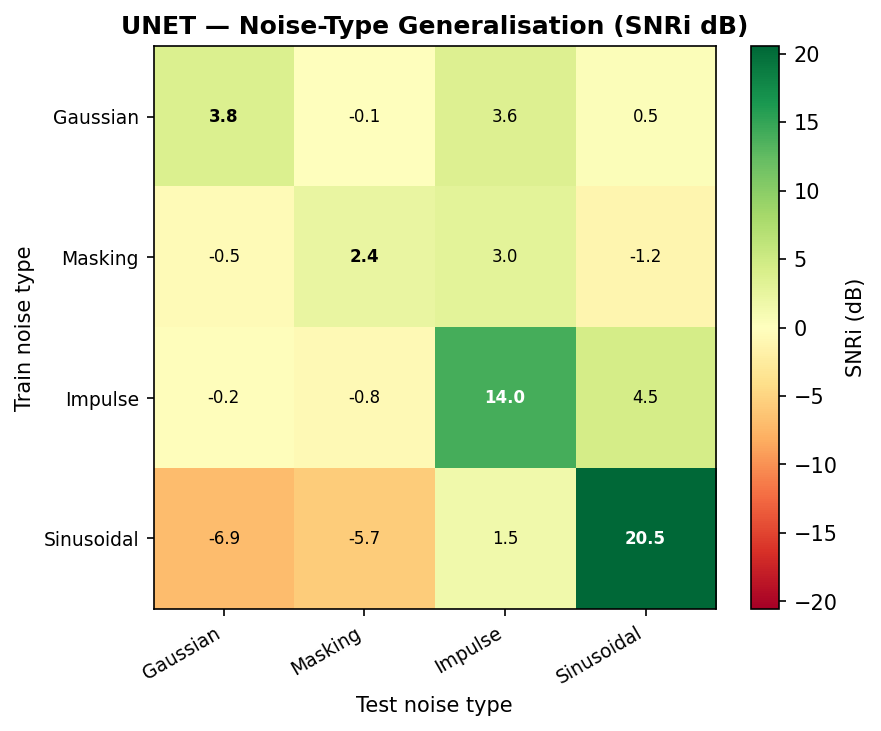
\includegraphics[width=0.49\linewidth]{assets/unet_noise_type_matrix.png}
\hfill
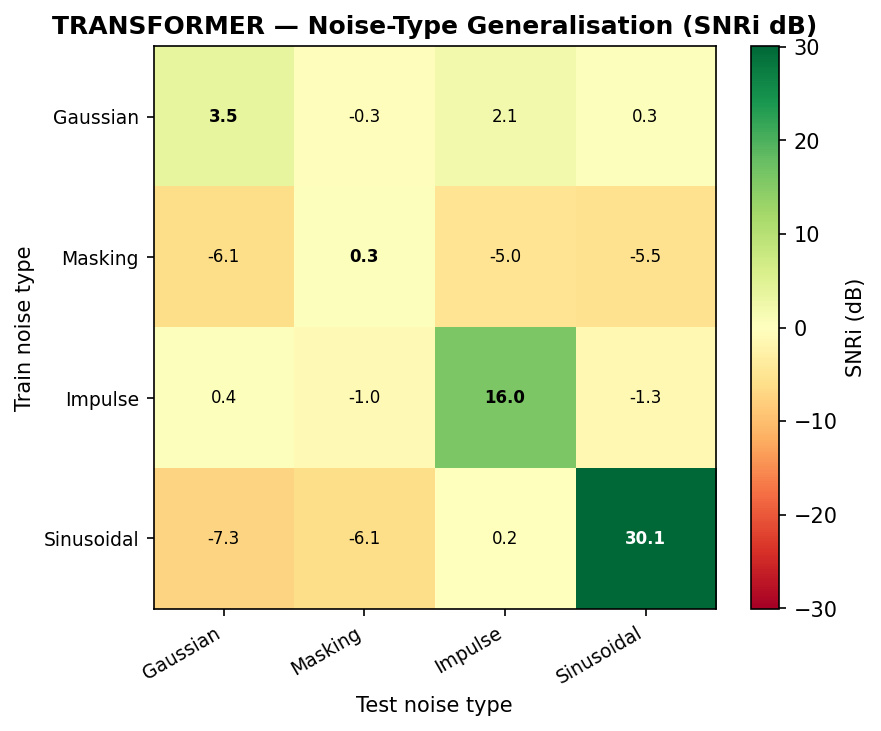
\includegraphics[width=0.49\linewidth]{assets/transformer_noise_type_matrix.png}
\end{center}
\vspace{-4pt}
\caption{SNRi heatmaps for the two successful architectures.
\textbf{Left}: UNet-1D. \textbf{Right}: Transformer.
Green\,=\,positive; red\,=\,negative. Diagonal = matched condition.}
\label{fig:noise-matrix}
\vspace{-4pt}
\end{figure}

\textbf{Analysis.}
Three structural patterns emerge.

\textbf{(i) Impulse noise yields positive SNRi for \emph{every} model}
regardless of training type---even FC on sinusoidal achieves $+7.4$\,dB on
impulse test data.
Impulse spikes are extreme outliers; any reconstruction that produces a smooth
output will suppress them automatically.

\textbf{(ii) Skip-connection models achieve large matched-condition SNRi on
specialised noises.}
UNet-1D: $+14.0$\,dB on impulse, $+20.5$\,dB on sinusoidal.
Transformer: $+16.0$\,dB on impulse, $+30.1$\,dB on sinusoidal
(Transformer's global attention is particularly effective at identifying and
suppressing the sharp spectral peak of the 5\,Hz tone).
However, this specialisation is costly: UNet trained on sinusoidal drops to
$-6.9$\,dB on Gaussian; Transformer to $-7.3$\,dB.

\textbf{(iii) Gaussian training is the most robust deployment strategy.}
UNet trained on Gaussian achieves ($+3.8$, $-0.1$, $+3.6$, $+0.5$)\,dB
across (Gaussian, masking, impulse, sinusoidal) tests;
Transformer achieves ($+3.5$, $-0.3$, $+2.1$, $+0.3$)\,dB.
All values are near-zero or positive.
For clinical deployment where noise composition is unknown, Gaussian training
is the recommended strategy.

% ════════════════════════════════════════════════════════════════════
\section{Discussion and Conclusion}
\label{sec:conclusion}

\textbf{Key finding: skip connections are necessary and sufficient.}
Across all five experiments, the presence of a skip connection bypass---not
the type of inductive bias (local, sequential, or global)---determines whether
a model can denoise wrist IMU signals at this dataset scale.
FC/CNN/LSTM all fail (negative SNRi) regardless of latent dimension, training
length, or noise type, because the 6144$\to$64 bottleneck introduces more
distortion than the injected noise.
UNet-1D (multi-scale spatial skip) and Transformer (patch-token skip) both
reach MSE\,$\approx 0.004$ and SNRi\,$\approx +5.4$\,dB across all tested
conditions.

\textbf{Clinical implications.}
TremorMAE is the decisive clinical metric: FC/CNN/LSTM inflate 4--6\,Hz band
distortion by 118--168$\times$, making downstream tremor severity assessment
unreliable even when MSE appears moderate.
UNet/Transformer keep TremorMAE below 0.68\,Hz$^2$.
For deployment with unknown noise composition, Gaussian-trained UNet-1D or
Transformer is the recommended configuration.

\textbf{Limitations.}
Noise is applied synthetically; real-world IMU artifacts are correlated and
non-stationary.
The dataset covers $\approx$247 of 355 subjects, limiting test-set statistical
power.
Noise-type cross-evaluation used only 20 epochs, so some cells may not have
fully converged.
No downstream tremor severity task was evaluated.

\textbf{Future work.}
Mixed-noise training (sampling the noise type per batch) is a natural next
step to close the specialisation--robustness gap.
Lightweight model distillation from Transformer to a smaller UNet variant
would enable edge deployment on the Apple Watch itself.

\subsubsection*{Author Contributions}

\textbf{Wanghley Soares Martins:}
Dataset integration (PADS loader, subject-level splitting, z-score
normalisation); UNet-1D and patch Transformer architectures; hybrid
time-frequency loss; LSTM encoder fix; noise-type cross-evaluation;
TremorMAE metric; system integration and paper writing.

\textbf{Yibei Gou:}
FC, CNN, and LSTM architectures; MSE/SNR evaluation pipeline; Adam
optimiser with scheduler and gradient clipping; hyperparameter grid search;
latent-dimension sweep; noise robustness experiment.

\bibliography{iclr2024_conference}
\bibliographystyle{iclr2024_conference}

\end{document}
